% ! TeX root = ../bachelor-thesis.tex

\chapter{Progettazione delle skill}
\label{ch:Chapter4}

In questo capitolo, si descriverà il processo di progettazione delle
\textit{skill} per i giochi cognitivi.

Più in dettaglio, per ciascuna \textit{skill}, sarà prima delineato l’esercizio
cognitivo implementato e il suo scopo, facendo riferimento alle capacità
cognitive di cui permette l’allenamento. Successivamente, se ne illustrerà un
caso d’uso specifico, che ne riassumerà i requisiti, ovvero la logica del gioco
implementato. Infine, sarà presentato il progetto di una sua possibile
soluzione, descrivendo i contesti in cui si può trovare l’utente nella
\textit{skill} e le intenzioni che può esprimere all’interno di tali contesti.

I giochi implementati avranno alcune caratteristiche in comune. Innanzitutto,
saranno giochi che, per come sono gestite le interazioni con Alexa, si
svolgeranno \textbf{necessariamente a turni}. Ogni turno, l’utente potrà
esprimere una propria volontà attraverso un’intenzione, che potrà essere
soddisfatta dall’endpoint, producendo una risposta adeguata da parte di Alexa.
Inoltre, si è deciso di seguire un \textbf{modello d'interazione simile} per
proseguire all’interno dei giochi della suite. In questo modo, una volta
raggiunto un certo livello di familiarità con uno specifico gioco, all’utente
risulterà più facile interagire con gli altri giochi. In particolare,
esisteranno dei comandi comuni nei giochi per conoscere le funzionalità della
\textit{skill}, le regole del gioco implementato e per cominciare una partita.

Altri comandi condivisi, sono invece comandi standard richiesti da Amazon per
poter eseguire il deployment di una \textit{skill}, come quelli per aprire e
chiudere la \textit{skill}.

\section{Number List Game}
\label{sec:Sezione4.1}

\textbf{Number List Game} è il primo gioco sviluppato per questa suite. È
stato utilizzato per sondare le capacità di un’assistente vocale nel contesto
dell’allenamento delle funzioni cognitive del cervello.

Il gioco consiste semplicemente nel dover ripetere una lista di numeri espressa
da Alexa. La lista di numeri cambia e diventa più lunga a ogni turno. Al primo
errore, il gioco termina, annunciando al giocatore il suo punteggio finale,
ovvero il numero di liste che è riuscito a ricordarsi correttamente.

Lo scopo del gioco è quello di allenare la \textbf{memoria a breve termine},
infatti sarà richiesto all’utente di ricordarsi una cosa sempre diversa e
sempre più difficile.

\subsection{Analisi del modello di dialogo}
\label{subsec:Sezione4.1.1}

Di seguito, viene riportata la progettazione di un esempio d'interazione tra
l’utente e la \textit{skill} Number List Game, che riassume i requisiti
fondamentali della \textit{skill}, ovvero la logica di base del gioco (Figura
\ref{fig:figure4.1}).

\begin{figure}[!ht]
  \centering
  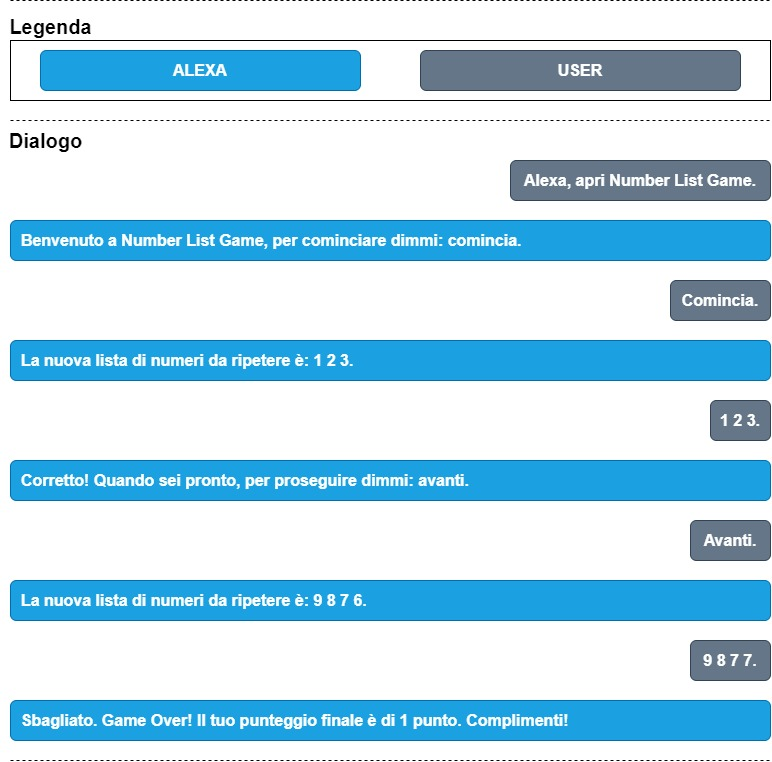
\includegraphics[scale=0.5]{resources/images/analysis/skill-flow-example/number-list-game-flow-example.jpg}
  \caption{
    Un esempio d'interazione con la \textit{skill} Number List Game,
    progettato per riassumere la logica del gioco.
  }
  \label{fig:figure4.1}
\end{figure}

\subsection{Progettazione del modello di dialogo}
\label{subsec:Sezione4.1.2}

Nel capitolo seguente, viene riportato il progetto di una possibile soluzione
che soddisfi i requisiti della \textit{skill} Number List Game. In particolare,
il progetto consiste in un diagramma di stati della \textit{skill}, in cui gli
stati sono da intendersi come \textbf{contesti} e \textbf{sotto-contesti}, in
cui ha senso esprimere una certa \textbf{intenzione} o meno. Il contesto in cui
si trova una \textit{skill} può cambiare in base alle intenzioni espresse
dall’utente. A ogni intenzione, corrisponde un’azione che sarà eseguita dalla
\textit{skill}.

\begin{figure}[!ht]
  \centering
  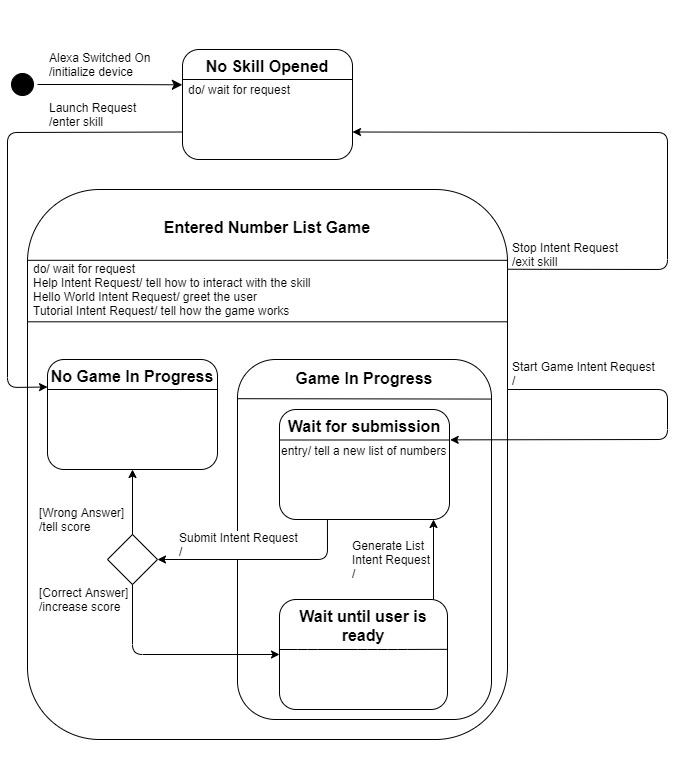
\includegraphics[scale=0.56]{resources/images/design/skill-state-diagram/number-list-game-state-diagram.jpg}
  \caption{Diagramma degli stati della \textit{skill} Number List Game.}
  \label{fig:figure4.2}
\end{figure}

Come si vede dalla Figura \ref{fig:figure4.2}, sarà possibile interagire con la
\textit{skill} attraverso le seguenti \textit{intenzioni}, all’interno degli
opportuni \textit{contesti} e \textit{sotto-contesti}:
\begin{itemize}
  \item \textbf{NO SKILL OPENED}: contesto in cui la skill non è ancora stata
        aperta; è anche il contesto in cui si trova Alexa subito dopo
        l’accensione:
        \begin{itemize}
          \item[o] \textit{\textbf{Launch Request}}: intenzione che esprime la
                volontà dell’utente di \textit{aprire la skill Number List
                Game};
        \end{itemize}
  \item \textbf{ENTERED NUMBER LIST GAME}: contesto in cui la skill è stata
        aperta:
        \begin{itemize}
          \item[o] \textit{\textbf{Stop Intent Request}}: intenzione che
                esprime la volontà dell’utente di \textit{uscire dalla skill
                Number List Game};
          \item[o] \textit{\textbf{Hello World Intent Request}}: intenzione che
                esprime la volontà dell’utente di \textit{essere salutato dalla
                skill Number List Game} (utilizzata per testare la
                comunicazione con la skill);
          \item[o] \textit{\textbf{Help Intent Request}}: intenzione che
                esprime la volontà dell’utente di \textit{conoscere com’è
                possibile interagire con la skill Number List Game};
          \item[o] \textit{\textbf{Tutorial Intent Request}}: intenzione che
                esprime la volontà dell’utente di \textit{conoscere come
                funziona il gioco};
          \item[o] \textit{\textbf{Start Game Intent Request}}: intenzione che
                esprime la volontà dell’utente di \textit{cominciare una nuova
                partita};
          \item[o] \textbf{NO GAME IN PROGRESS}: contesto in cui non è ancora
                stata cominciata nessuna partita;
          \item[o] \textbf{GAME IN PROGRESS}: contesto in cui è già in corso
                una partita:
                \begin{itemize}
                  \item[•] \textbf{WAIT FOR SUBMISSION}: contesto in cui la
                        skill ha comunicato una lista di numeri e aspetta che
                        l’utente la ripeti:
                        \begin{itemize}
                          \item[o] \textit{\textbf{Submit Intent Request}}:
                                intenzione che esprime la volontà
                                d'\textit{inviare una lista di numeri alla
                                skill};
                        \end{itemize}
                  \item[•] \textbf{WAIT UNTIL USER IS READY}: contesto in cui
                        la skill ha processato il tentativo corretto
                        dell’utente di ripetere la lista di numeri
                        precedentemente comunicata e aspetta una conferma da
                        parte del giocatore:
                        \begin{itemize}
                          \item[o] \textit{\textbf{Generate List Intent
                                Request}}: intenzione che esprime la volontà di
                                \textit{ricevere una nuova lista di numeri da
                                ripetere}.
                        \end{itemize}
                \end{itemize}
        \end{itemize}
\end{itemize}

\section{Category Game}
\label{sec:Sezione4.2}

Un altro gioco sviluppato per questa suite è \textbf{Category Game}. Il gioco
consiste nel categorizzare le parole comunicate da Alexa. In particolare,
possiede due diverse modalità:

\begin{itemize}
  \item[--] Nella \textit{modalità facile}, Alexa comunicherà al giocatore una
        categoria. Successivamente, a ogni turno, riferirà una parola diversa
        che il giocatore dovrà indicare come appartenente alla categoria o meno.
        Lo scopo della modalità è quello di allenare l’\textbf{attenzione} e la
        \textbf{categorizzazione}, infatti sarà richiesto all’utente di
        riconoscere solo alcune parole, tra tutte, come appartenenti a un
        certo gruppo;
  \item[--] Nella \textit{modalità difficile}, Alexa comunicherà al giocatore
        due categorie. Dopodiché, a ogni turno, riferirà una parola diversa
        appartenente a una delle due categorie menzionate. In questo caso però,
        il giocatore dovrà indicare la parola come appartenente alla categoria
        contraria a quella corretta.
        Lo scopo della modalità è quello di allenare l’\textbf{attenzione} e
        l’\textbf{inibizione degli automatismi}, infatti sarà richiesto
        all’utente di andare contro le sue abitudini e di rispondere in modo
        errato ai quesiti posti.
\end{itemize}

Il gioco termina al primo errore commesso dal giocatore, annunciando il suo
punteggio finale, ovvero il numero di parole che è riuscito a categorizzare
correttamente.

\subsection{Analisi del modello di dialogo}
\label{subsec:Sezione4.2.1}

Di seguito, viene riportata la progettazione di due esempi d'interazione tra
l’utente e la \textit{skill} Category Game, uno per modalità di gioco (Figura
\ref{fig:figure4.3} e Figura \ref{fig:figure4.4}). \newpage

\begin{figure}[!h]
  \centering
  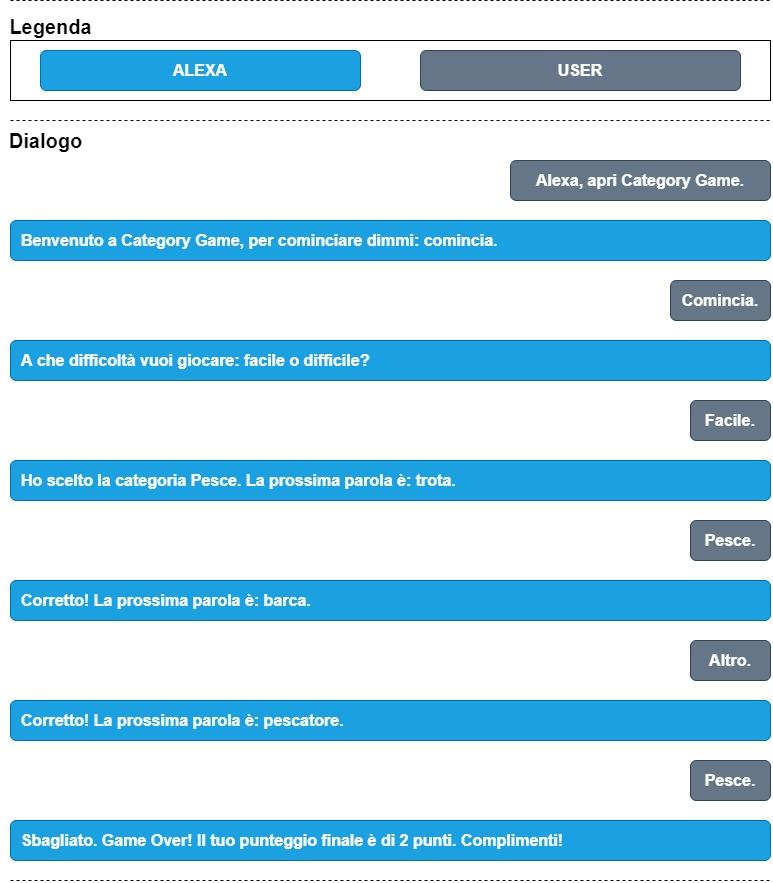
\includegraphics[scale=0.5]{resources/images/analysis/skill-flow-example/category-game-flow-example-easy.jpg}
  \caption{
    Esempio d'interazione con la \textit{skill} Category Game, progettato per
    riassumere la logica del gioco nella modalità facile.
  }
  \label{fig:figure4.3}
\end{figure}
\newpage

\begin{figure}[!h]
  \centering
  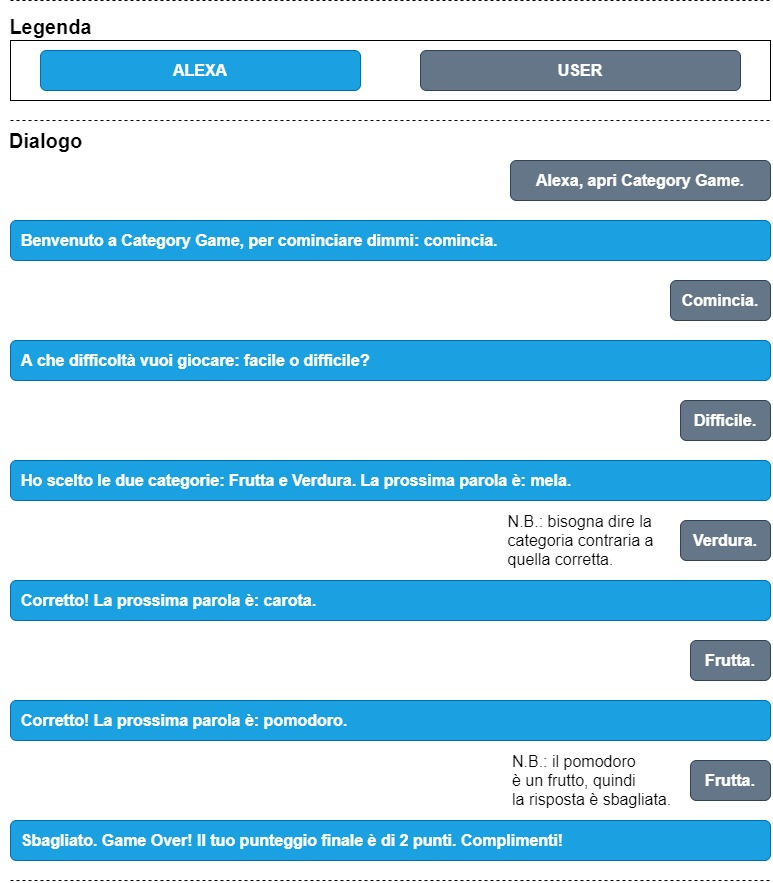
\includegraphics[scale=0.5]{resources/images/analysis/skill-flow-example/category-game-flow-example-difficult.jpg}
  \caption{
    Esempio d'interazione con la \textit{skill} Category Game, progettato per
    riassumere la logica del gioco nella modalità difficile.
  }
  \label{fig:figure4.4}
\end{figure}
\newpage

\subsection{Progettazione del modello di dialogo}
\label{subsec:Sezione4.2.2}

Ora viene riportato il progetto di una possibile soluzione che soddisfi i
requisiti della \textit{skill} Category Game.

\begin{figure}[!ht]
  \centering
  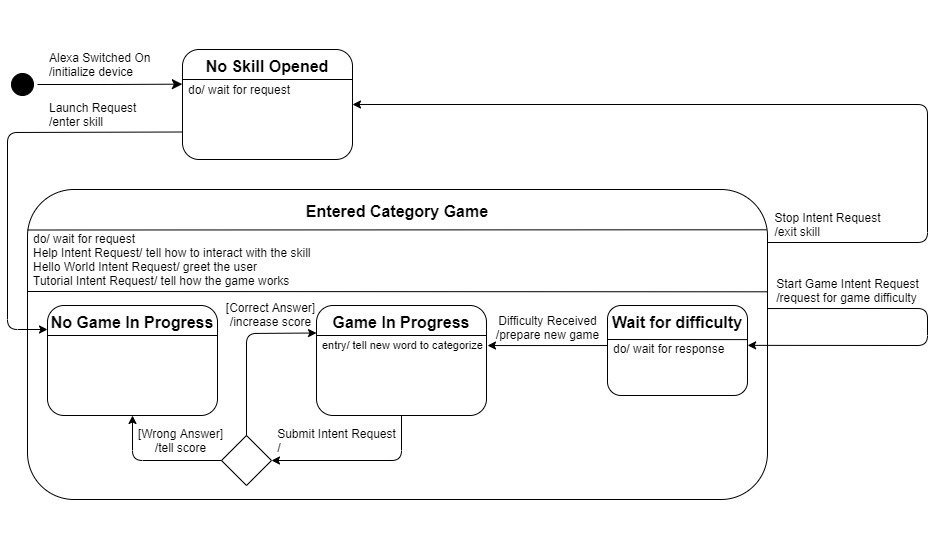
\includegraphics[scale=0.48]{resources/images/design/skill-state-diagram/category-game-state-diagram.jpg}
  \caption{Diagramma degli stati della \textit{skill} Category Game.}
  \label{fig:figure4.5}
\end{figure}

Come si vede dalla Figura \ref{fig:figure4.5}, sarà possibile interagire con la
\textit{skill} attraverso le seguenti \textit{intenzioni}, all’interno degli
opportuni \textit{contesti} e \textit{sotto-contesti}:
\begin{itemize}
  \item \textbf{NO SKILL OPENED}: contesto in cui la skill non è ancora stata
        aperta; è anche il contesto in cui si trova Alexa subito dopo
        l’accensione:
        \begin{itemize}
          \item[o] \textit{\textbf{Launch Request}}: intenzione che esprime la
                volontà dell’utente di \textit{aprire la skill Category Game};
        \end{itemize}
  \item \textbf{ENTERED NUMBER LIST GAME}: contesto in cui la skill è stata
        aperta:
        \begin{itemize}
          \item[o] \textit{\textbf{Stop Intent Request}}: intenzione che
                esprime la volontà dell’utente di \textit{uscire dalla skill
                Category Game};
          \item[o] \textit{\textbf{Hello World Intent Request}}: intenzione che
                esprime la volontà dell’utente di \textit{essere salutato dalla
                skill Category Game} (utilizzata per testare la comunicazione
                con la skill);
          \item[o] \textit{\textbf{Help Intent Request}}: intenzione che
                esprime la volontà dell’utente di \textit{conoscere com’è
                possibile interagire con la skill};
          \item[o] \textit{\textbf{Tutorial Intent Request}}: intenzione che
                esprime la volontà dell’utente di \textit{conoscere come
                funziona il gioco};
          \item[o] \textit{\textbf{Start Game Intent Request}}: intenzione che
                esprime la volontà dell’utente di \textit{cominciare una nuova
                partita}. In questo caso, prima di cominciare la partita, sarà
                richiesto all’utente di specificare anche la difficoltà a cui
                vuole giocare, che sarà utilizzata per determinare la modalità
                di gioco;
          \item[o] \textbf{NO GAME IN PROGRESS}: contesto in cui non è ancora
                stata cominciata nessuna partita;
          \item[o] \textbf{GAME IN PROGRESS}: contesto in cui è già in corso
                una partita ed è stata comunicata una parola da categorizzare
                al giocatore:
                \begin{itemize}
                  \item[•] \textit{\textbf{Submit Intent Request}}: intenzione
                        che esprime la volontà del giocatore
                        d'\textit{inviare una categoria alla skill}.
                \end{itemize}
        \end{itemize}
\end{itemize}

Si noti come in questo caso si sia deciso di non richiedere ogni turno la
conferma per proseguire nel gioco. Questa decisione è stata presa per
alleggerire il flusso di dialogo e diminuire il numero d'interazioni necessarie
per progredire in una partita.

\section{Labyrinth Game}
\label{sec:Sezione4.3}

\textbf{Labyrinth Game} è il gioco più complesso sviluppato per questa suite.

Il gioco consiste nel doversi muovere e orientare all’interno di un labirinto
bidimensionale, raggiungendone eventualmente l’uscita. All’inizio della
partita, Alexa genererà il labirinto. Successivamente, a ogni turno, Alexa
descriverà i dintorni del giocatore, il quale dovrà scegliere una direzione
verso cui spostarsi.

Come mostrato nella Figura \ref{fig:figure4.6}, il labirinto sarà composto di:
\begin{itemize}
  \item[--] \textit{Mura}: componenti non attraversabili;
  \item[--] \textit{Mura di perimetro}: componenti non attraversabili, che
        costituiscono il perimetro del labirinto;
  \item[--] \textit{Percorsi}: componenti attraversabili;
  \item[--] \textit{Torri}: componenti attraversabili, che forniscono dei
        suggerimenti al giocatore per aiutarlo a raggiungere l’uscita del
        labirinto;
  \item[--] \textit{Un’entrata}: il percorso su cui si trova il giocatore
        all’inizio della partita;
  \item[--] \textit{Un’uscita}: il percorso che dovrà raggiungere il giocatore
        per terminare la partita.
\end{itemize}
\begin{figure}[!ht]
  \centering
  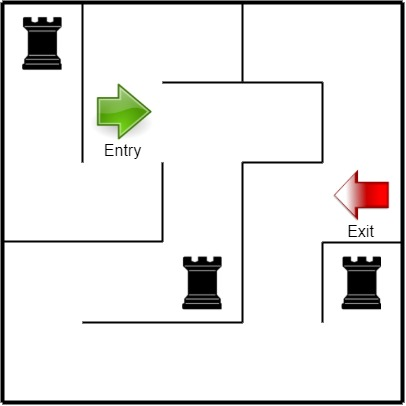
\includegraphics[scale=0.5]{resources/images/other/labyrinth-game-labyrinth-example.jpg}
  \caption{
    Esempio di layout di un labirinto nella \textit{skill} Labyrinth Game.
  }
  \label{fig:figure4.6}
\end{figure}

Il gioco termina quando il giocatore raggiunge l’uscita del labirinto,
annunciando il suo punteggio finale, ovvero il numero di passi che ha compiuto
prima di raggiungere l’uscita.

Lo scopo del gioco è quello di allenare la \textbf{memoria a lungo termine},
l’\textbf{orientamento} e l’\textbf{immaginazione}, infatti sarà richiesto
all’utente di ricordare e costruirsi mentalmente il layout del labirinto man
mano che lo esplora, riconoscendo la posizione in cui si trova.

\subsection{Analisi del modello di dialogo}
\label{subsec:Sezione4.3.1}

Di seguito, viene riportata la progettazione di un esempio d'interazione
dell’utente con la \textit{skill} Labyrinth Game (Figura \ref{fig:figure4.7}).
\newpage

\begin{figure}[!ht]
  \centering
  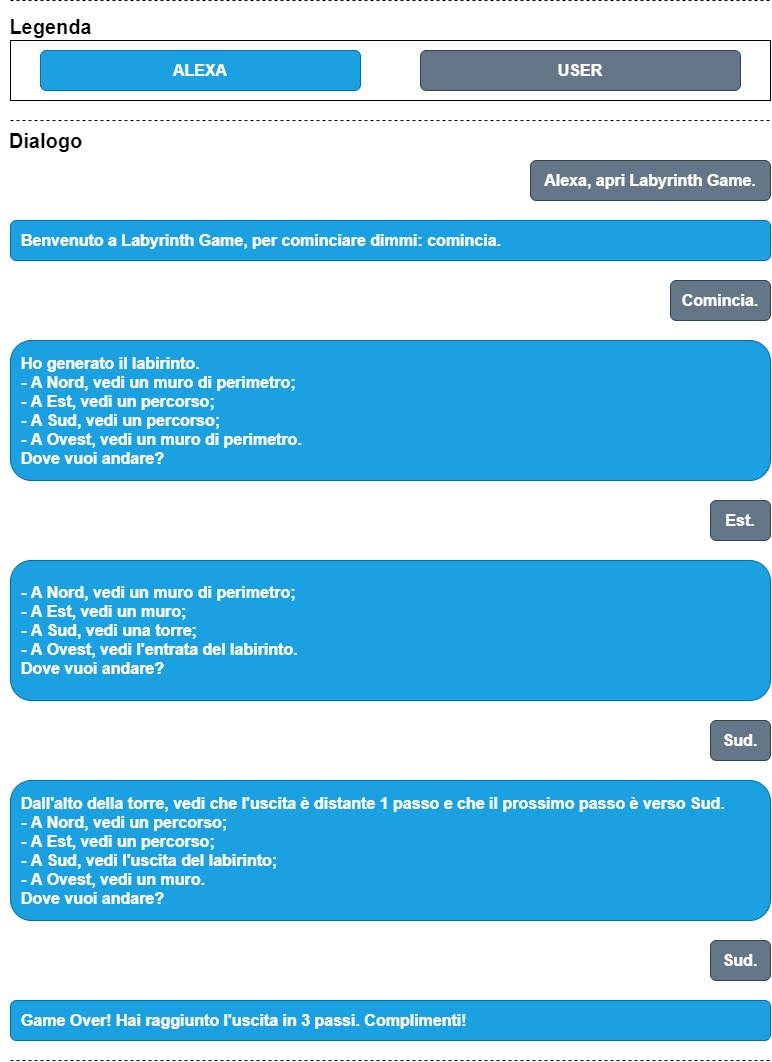
\includegraphics[scale=0.5]{resources/images/analysis/skill-flow-example/labyrinth-game-flow-example.jpg}
  \caption{
    Esempio d'interazione con la \textit{skill} Labyrinth Game, progettato per
    riassumere la logica del gioco.
  }
  \label{fig:figure4.7}
\end{figure}
\newpage

\subsection{Progettazione del modello di dialogo}
\label{subsec:Sezione4.3.2}

Ora viene riportato il progetto di una possibile soluzione che soddisfi i
requisiti della \textit{skill} Labyrinth Game.

\begin{figure}[!ht]
  \centering
  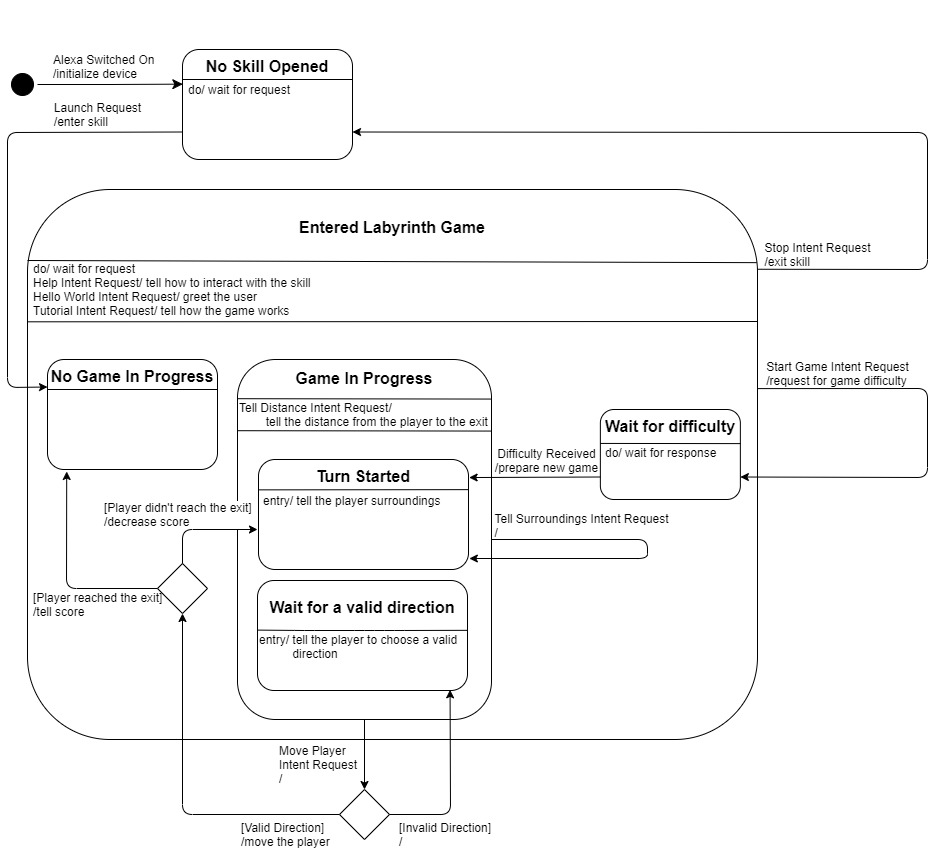
\includegraphics[scale=0.48]{resources/images/design/skill-state-diagram/labyrinth-game-state-diagram.jpg}
  \caption{Diagramma degli stati della \textit{skill} Labyrinth Game.}
  \label{fig:figure4.8}
\end{figure}

Come si vede dalla Figura \ref{fig:figure4.8}, sarà possibile interagire con la
\textit{skill} attraverso le seguenti \textit{intenzioni}, all’interno degli
opportuni \textit{contesti} e \textit{sotto-contesti}:
\begin{itemize}
  \item \textbf{NO SKILL OPENED}: contesto in cui la skill non è ancora stata
        aperta; è anche il contesto in cui si trova Alexa subito dopo
        l’accensione:
        \begin{itemize}
          \item[o] \textit{\textbf{Launch Request}}: intenzione che esprime la
                volontà dell’utente di \textit{aprire la skill Labyrinth Game};
        \end{itemize}
  \item \textbf{ENTERED NUMBER LIST GAME}: contesto in cui la skill è stata
        aperta:
        \begin{itemize}
          \item[o] \textit{\textbf{Stop Intent Request}}: intenzione che
                esprime la volontà dell’utente di \textit{uscire dalla skill
                Labyrinth Game};
          \item[o] \textit{\textbf{Hello World Intent Request}}: intenzione che
                esprime la volontà dell’utente di \textit{essere salutato dalla
                skill Labyrinth Game} (utilizzata per testare la comunicazione
                con la skill);
          \item[o] \textit{\textbf{Help Intent Request}}: intenzione che
                esprime la volontà dell’utente di \textit{conoscere com’è
                possibile interagire con la skill Labyrinth Game};
          \item[o] \textit{\textbf{Tutorial Intent Request}}: intenzione che
                esprime la volontà dell’utente di \textit{conoscere come
                funziona il gioco};
          \item[o] \textit{\textbf{Start Game Intent Request}}: intenzione che
                esprime la volontà dell’utente di \textit{cominciare una nuova
                partita}. Prima di cominciare la partita, sarà richiesto
                all’utente di specificare anche la difficoltà a cui vuole
                giocare, che sarà utilizzata per determinare le dimensioni del
                labirinto;
          \item[o] \textbf{NO GAME IN PROGRESS}: contesto in cui non è ancora
                stata cominciata nessuna partita;
          \item[o] \textbf{GAME IN PROGRESS}: contesto in cui è già in corso
                una partita ed è stato generato il labirinto su cui giocherà
                l’utente:
                \begin{itemize}
                  \item[•] \textit{\textbf{Tell Distance Intent}}: intenzione
                        che esprime la volontà del giocatore di
                        \textit{conoscere la sua distanza dall’uscita};
                  \item[•] \textbf{TURN STARTED}: contesto in cui sono già
                        stati descritti i dintorni del giocatore:
                        \begin{itemize}
                          \item[o] \textit{\textbf{Tell Surroundings Intent}}:
                                intenzione che esprime la volontà del giocatore
                                di \textit{conoscere i propri dintorni};
                          \item[o] \textit{\textbf{Move Player Intent}}:
                                intenzione che esprime la volontà del giocatore
                                di \textit{muoversi verso una certa direzione}.
                        \end{itemize}
                \end{itemize}
        \end{itemize}
\end{itemize}

A questo punto, una volta presentato il progetto, è possibile passare alla
descrizione della sua effettiva implementazione.